\documentclass[11pt, oneside]{article}
\usepackage{listings}
\usepackage{amsmath}
\usepackage{graphicx}
\usepackage{subfigure}
\usepackage{float}
\usepackage[margin=1in]{geometry}

\newcommand{\fref}[1]{Figure~\ref{#1}}

\begin{document}
\title{Memory and Data Access Privacy}
\author{
    \makebox[.25\linewidth]{Ken Cheng} \and
    \makebox[.25\linewidth]{Nick Dryanovsky} \and
    \makebox[.25\linewidth]{Devan Lai} \and
    \makebox[.25\linewidth]{Kevin Morgan} \and
    \makebox[.25\linewidth]{Hugh Oh} \and
    \makebox[.25\linewidth]{Kevin Porter} \and
    \makebox[.25\linewidth]{Jacob Privalsky} \and
    \makebox[.25\linewidth]{Adarsh Ramakrishnan} \and
    \makebox[.25\linewidth]{Rafael Send}
}
\date{\today}
\maketitle

\begin{abstract}
In this paper, we explore a novel way of invading computer-usage privacy. By
examining the memory addresses of the requests to RAM and hard drive, we show
that it is possible to extract information about the program that is running.
\end{abstract}

%\setcounter{section}{-1}
\section{Introduction}
With the popularization of virtualization technologies and decreasing cost of 
server co-location maintenance, an increasing number of servers are being 
moved to third party managed virtual machines somewhere on the cloud. While 
this modern approach to solving the economic dilemma of controlling company 
revenue spend    on on-site technical staff does contain attractive benefits, 
it unfortunately opens the door to many complications that are introduced in 
the process of preserving the integrity of sensitive customer data in a 
potentially hostile IT environment. As a result, the field of providing easy 
to implement fundamental precautionary solutions for the protection of 
confidential information is continuously developing and encryption of data 
transfer channels finds it place at the heart of the most essential toolkit 
that is available to every system administrator. Unfortunately, while 
encryption can certainly provide a level of data integrity protection, the 
fact that server physical access is available to maintenance technical staff 
that could be considered an untrusted source that can exploit its practically 
unlimited physical access to the hardware raises the issues of examining the 
efficiency of data encryption against hardware related attacks. In particular 
we would focus on the case where the previously mentioned untrusted party 
represented by the co-location technical staff is able to successfully install 
a hardware device that is able to record memory and disk requests. This device 
could then be exploited by the attacker to obtain actionable intelligence 
about the inner working of specific applications on the clients server.

\section{Overview}
To obtain sensitive information from a particular application through the 
exploitation of \textbf{memory traces}\footnote{Requested memory addresses 
that missed in the lowest level of cache, along with the associated type of 
request (instruction read, data read, data write).} and 
\textbf{disk traces}\footnote{Block read/write requests}, an attacker must 
first be able to fingerprint the application of interest and recognize or 
compile a set of data related to the targeted application's normal operational 
behaviors. Once such dataset of application specific actions has been 
generated, a potential attacker would have a sufficient foundation to explore 
various data mining techniques by which he/she might be able to compare, 
match, analyze and eventually extract viable information from the signature 
traces from the targeted machine.

For this project, we gathered information using the software tools Cachegrind
and blktrace rather than tampering into actual hardware. In addition, we 
assumed single processes running on single CPUs. Depending on the program that 
we chose to attack, we developed different ways of analyzing the traces to
form possible attacks, which we discuss further in the following sections.


\section{SVN Version Control Analysis}
\subsection{Application Overview}
We chose an SVN server as the application to analyze.  An attack on our 
application would constitute being able to determine which SVN commands are 
being performed at a given time or which or how many files are being modified. 
Due to the nature of our application, we decided that a disk trace would bear 
more fruitful results and would be more helpful in determining if our 
application could be attacked. The disk tracing utility that we used to gather 
our data {\tt blktrace} provided us with a disk trace while the SVN server 
executed some command.  However, we had to simulate the SVN server commands on 
our own on an Amazon EC2 instance. The output of blktrace contains the 
location and size of disk reads and writes each associated with a timestamp 
and process name.
\subsection{Analysis Process}
To provide a dataset for our tests we wrote a series of scripts to generate 
files of specified number and size with randomized data taken from /dev/
urandom. We primarily considered files in the size range 1-10KB, which we 
settled on as a reasonable approximation of the size of source files, which 
would be placed under version control in practice. We traced operations on 
data sets as small as one file and as large as 1000. By clearing the file 
system cache and filtering for traces originating from the SVN server, we were 
able to recover a detailed record of the disk operations requested by SVN.
\subsection{Tools and Results}
Our method of analyzing the traces was different from the other groups’ 
because we did not rely on the addresses of our disk accesses in order to 
determine the locality of the files being accessed. Instead of this, we tried 
to establish access patterns by looking at the individual operations 
themselves.  In our case, we were dealing with different files in different 
locations, and since modifying the files results in reading/writing a large 
disk block, it was difficult to find consistent locality patterns. Due to this 
difference, we opted to establish disk access patterns by looking at the 
individual operations of the traces and comparing chunks of these operations 
present between traces to determine differences between commands.

We were able to come up with a few vulnerabilities in the SVN server as well 
as the attacks that are a result of these vulnerabilities. We were fairly 
successful in distinguishing between SVN commands. Our basic approach was to 
analyze the number of reads versus writes over time, both by dividing the 
trace into segments and calculating read/write percentages and by simply 
graphing reads and writes over time. We were able to distinguish read-heavy 
commands such as checkout from write-heavy commands such as add. We were also 
able to find a very distinctive pattern characteristic of the delete command, 
allowing us to distinguish deletes from other mixed read/write operations. We 
attempted to find a relationship between the number of SVN IO requests 
necessitating disk seeks and the number of files being transferred or updated, 
but the correlation proved to be weak at best and results varied excessively 
with repeated trials. This may have been the result of file system 
fragmentation, interference from non-SVN processes, or access pattern 
optimizations beyond our direct control.

\begin{figure}[H]
    \centering
    \subfigure{
    	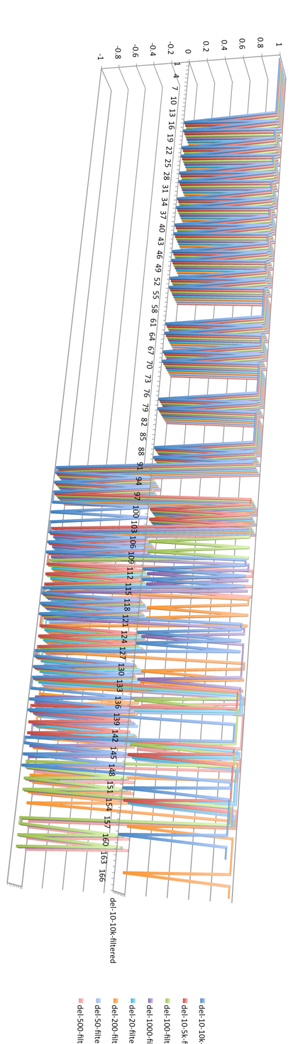
\includegraphics[height=7.6in]{SVN_left.png}
	    \label{fig:svn_left}
	}
	\subfigure{
	    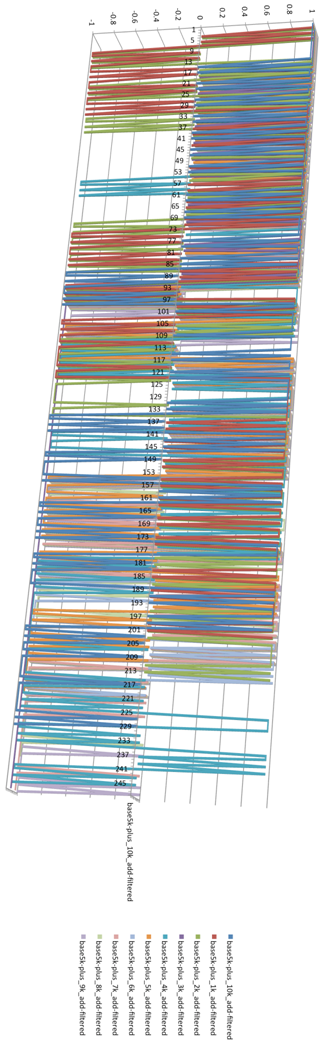
\includegraphics[height=7.6in]{SVN_right.png}
	    \label{fig:svn_right}
	}
	\caption{Disk access graphs}
	\label{fig:svn_graphs}
\end{figure}

\fref{fig:svn_left} compares delete traces of different file sizes (the sizes 
can be seen in the legend on the right).  The y-axis indicates whether the 
operation within the trace is a read (1), write (-1) or disk idle time (0). 
The x-axis indicates the line number of the delete traces filtered for IO 
requests generated by the SVN server. The fact that many of the operations of 
the traces overlap in chunks at the beginning shows us that regardless of the 
file size, these chunks of operations should be common to all delete traces. 
We can use this distinctive pattern to differentiate the delete command from 
the other SVN commands.

\fref{fig:svn_right} compares the traces of a 5kB size file and the same file 
with 1-10kB of random data added to the end of the file. The x and y axis on 
this graph represent the same things as in the previous one. These files 
represent the effect of committing changes to a file. Comparing the two graphs 
we can see that the first halves of both bear similarities in the chunks of 
reads that overlap between traces. However, in the second half of the right 
graph, we see that there is a large amount of noise as well as a substantial 
number of reads (as supposed to the first graph of the delete traces which had 
a large number of writes in its second half). Therefore, this difference in 
the second half of the graph enables us to differentiate between a 
differential commit and a delete command (given our data set).

\section{IRC Server Analysis}
\subsection{Application Overview}
This part of the project focused on an IRC daemon and its memory access 
patterns. Although IRC is not a particularly secure means of communication, we 
feel that this attack is representative of a class of attacks that could be 
applied to most programs. Our attack on Dancer-IRCD should be regarded as a 
proof-of-concept.

We made an attempt to identify common tasks users perform when interacting 
with the server. If we can identify commands being run on an IRC server, then 
it should be possible to identify commands being run on other application 
servers. The tests were performed on Dancer-IRCD, a relatively common IRC 
server. We used the modified version of chachegrind to record memory accesses. 
In particular, we collected memory traces for seven commands: connect, list, 
create room, quit, join, kick, and part. We then created a classification 
algorithm that was able to correctly predict all unknown commands from a 
validation set.

\subsection{Analysis Process}
The first challenge we faced was that the IRC server fit almost completely in 
the CPU cache. We had to reduce the cache size used by Valgrind to 32KB level 
1 instruction and data caches, and a 64 KB level 2 cache in order to get 
meaningful results, since with any larger size cache we were not able to get 
any memory accesses in some situations.

Initially, we had written a simple IRC client that played random messages of 
varying lengths onto the server and recorded the results automatically, but we 
found that we could not conduct meaningful analysis on the data collected this 
way. Instead, we realized that it would be more efficient to generate  memory 
traces for each command we were going to try and detect. This was done 
manually using an existing IRC client (irssi), where we repeatedly executed 
the same commands and recorded the corresponding accesses. 

We trained our command classifier on a set of memory traces corresponding to 
that command. For each command we took the intersection of the memory 
addresses from the traces in that command's training set. Our first attempt at 
classification was to take the intersection of the trace from an unknown 
command, and the subset associated with a command. Whichever command had the 
highest ratio (matched addresses/total addresses) was declared to match.

An issue occurred when a command had few identifying features that were 
contained in a larger set of features for another command. The algorithm would 
classify the trace as the command with the smaller feature set, even though 
the trace actually corresponded to the command with the larger feature set. 

To solve this problem, we realized that it would make sense to start with the 
largest feature set first. If a match was found for a large command set with a 
certainty above a specified threshold, the algorithm would stop searching and 
declare a command found. If no command reached the threshold, the highest 
rated command would be used. We set the threshold at 0.75, based on trends we 
saw in the data. In almost all cases, if a command was matched with at least 
0.75 accuracy, then it was likely correct. Another way to address this issue 
was to increase the training set size. With a training set of ten memory 
traces per command, this issue became negligible.

\subsection{Tools and Results}
From the data that the matching program output, we generated graphs to 
visualize our results. The program runs the intersecting set for each command 
against command to be classified, and outputs a likelihood for the commands. 
The largest of these is the matching result in most cases. However, very 
occasionally there would be more than one commands with equal probabilities, 
or values above the cutoff. For these, the solution was to sort by size and 
pick the larger one, as described in the analysis section. The sample shown 
below illustrates the issue, where both join and create room have the same 
probabilities.

The rest of the graphs show examples of the respective commands, where we did 
not strictly require the sorting part of the process to obtain the correct 
result.

We were able to correctly classify 69/70 of the commands in the verification 
set. We classified create room with 90\% accuracy, and all other commands with 
100\% accuracy. For the probabilites assigned to each command, see irc\_
results.odg in the supplemental code submission.

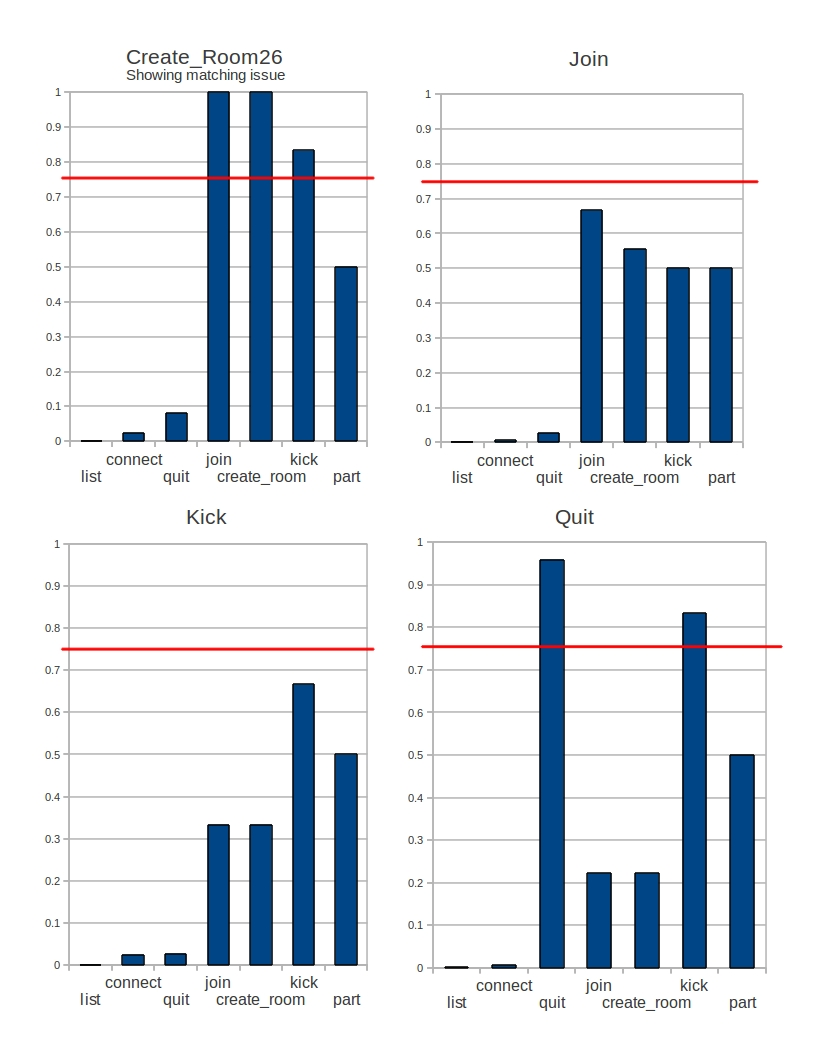
\includegraphics[height=6.47in, width=5in]{irc1.jpg}\\
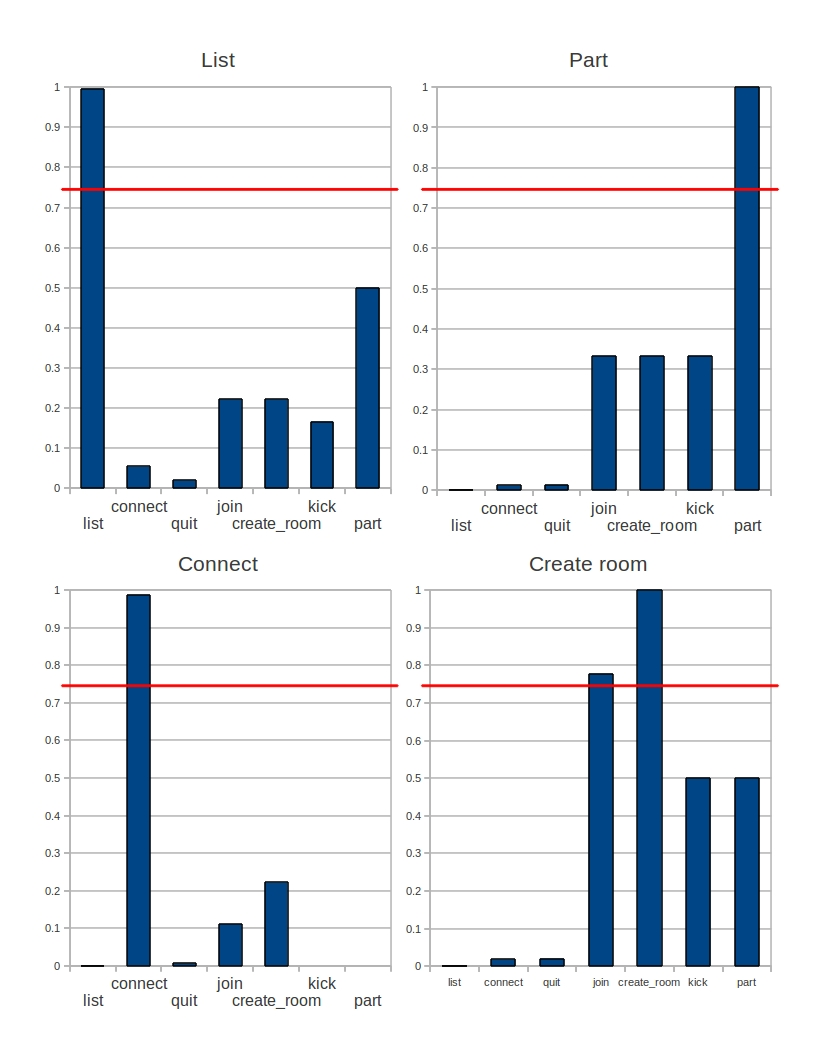
\includegraphics[height=6.47in, width=5in]{irc2.jpg}

\subsection{Conclusion}
We were able to successfully recognize all seven commands we issued to an IRC 
server with a high degree of accuracy, while using only a simulation of the 
addresses available on the memory bus. However, to achieve this, we had to 
decrease the cache size so that we could observe memory accesses. To 
extrapolate from this result, a memory bus based attack seems possible for 
programs that have executables significantly larger than that of Dancer-IRCD. 

\section[Squid Proxy Analysis]{Squid\footnote{Version 3.1} Proxy Analysis}
\subsection{Application Overview}
Web proxies can improve performance by caching commonly visited websites 
into memory or disk and retrieving the web page data on subsequent requests 
to that page. It is this functionality that we hope to use in an attack. On 
cache misses, we should see memory accesses to store the resources. On 
cache hits, we expect to see memory accesses back to the previously visited
address. If we can figure out this mapping from memory location to resource,
we would be able to figure out when someone is accessing a specific resource, 
like a site-key image. This attack would completely bypass the TLS protection
that makes HTTPS secure.

We chose Squid over other web proxies because it is widely available and well 
known. In addition, Squid is open source and can run as a single process 
daemon, which makes it easier (for us) to analyze the memory traces.

\subsection{Attack Strategy}
Our proposed strategy was to start Squid with an empty cache, access a web 
page, and figure out which memory addresses were accessed. Then we would
access a new web page and find the memory addresses unique to each request. 
From this we should be able to generate features unique to those web pages.
To prevent the CPU cache from storing everything internally, we flood the
CPU cache with a large sequence of HTTP requests in between accesses.

By reading the documentation on Squid, we found out that Squid caches objects
both in-memory and on-disk, so we gathered both memory traces
and disk traces.

\subsection{Memory Traces}
We first looked for a correlation between requests to the proxy and memory
accesses. Our primary test workload consisted of two cases---one where
a client accessed a sequence of Wikipedia articles resulting in only cache
misses and one where a client accessed a sequence of Wikipedia articles
twice, resulting in a sequence of misses followed by a sequence of hits.

Unfortunately, when we first collected traces, we discovered that due to
the large CPU cache size, there were almost no accesses to main memory
after Squid finished initialization. In a real attack, this would be less
of an issue as the cache would be invalidated by context-switching and
would be under greater load; in order to simulate this, we decreased the
effective L2 cache size from 8MiB to 64KiB.

Running the traces again, we were able to get a more representative view
of Squid's memory access pattern, as shown in \fref{fig:smash}.

\begin{figure}[h]
    \centering
    \subfigure[Memory pattern after accessing 100 Wikipedia sites] {
    	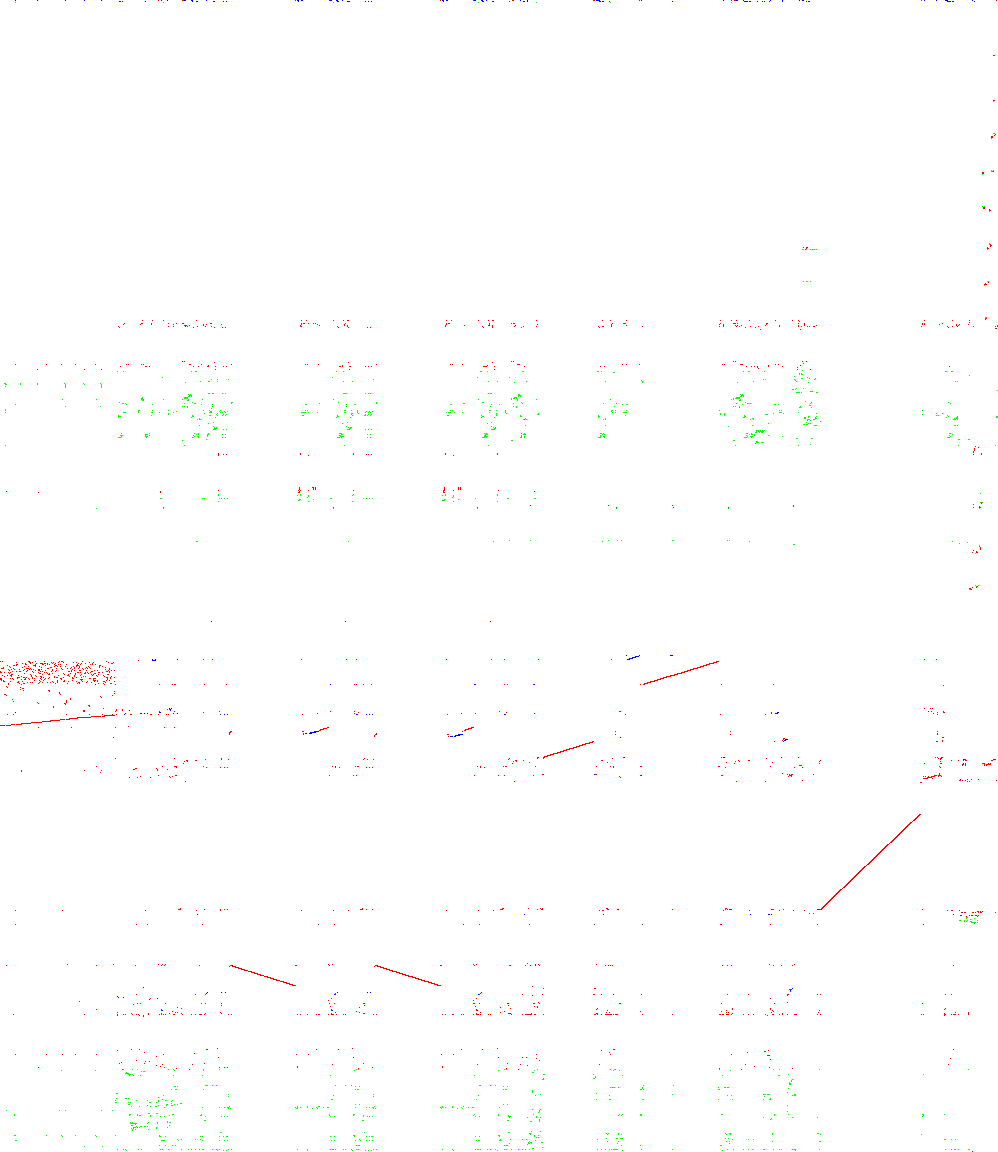
\includegraphics[width=3in]{smash5.png}
	    \label{fig:smash5}
	}
	\subfigure[Memory pattern after accessing 100 Wikipedia sites, and 
	then hitting the same 100 sites again.] {
	    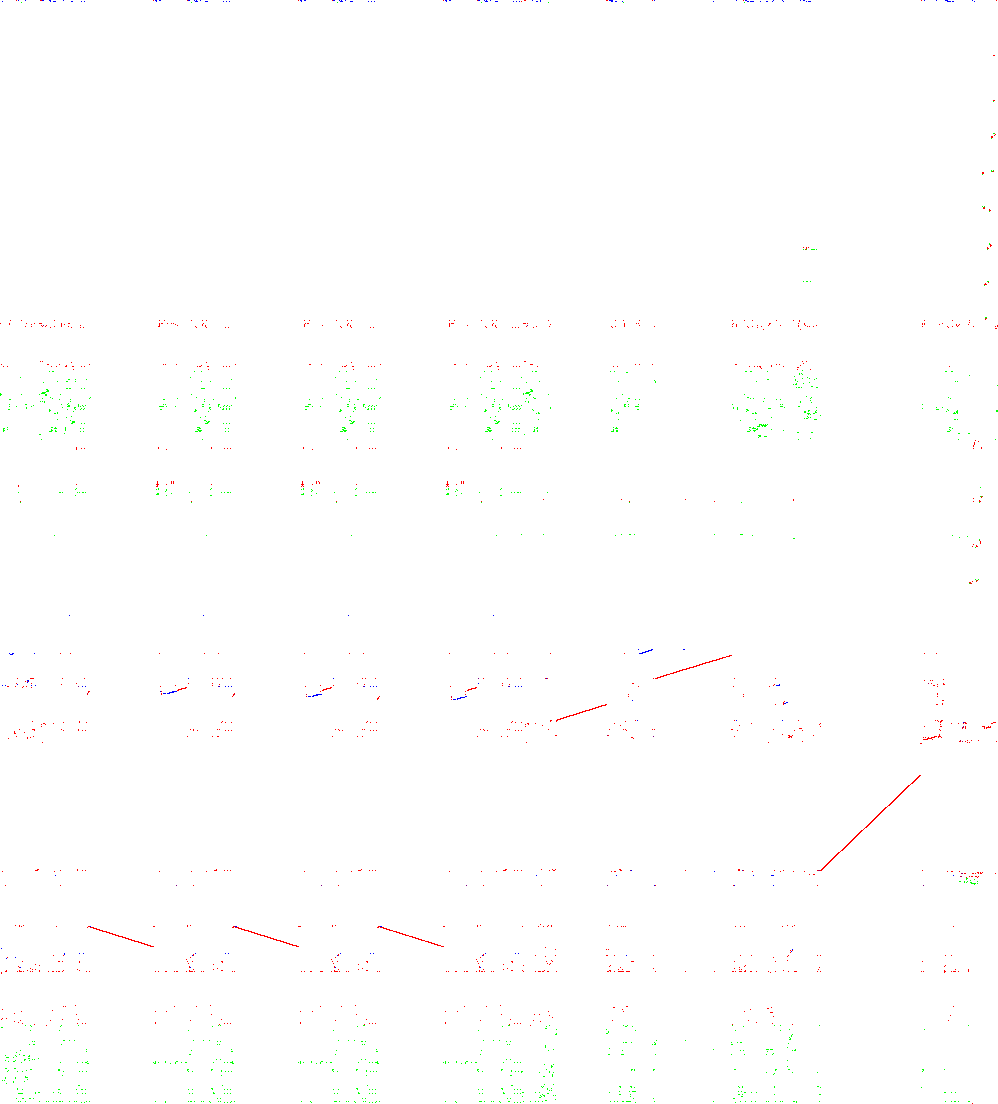
\includegraphics[width=3in]{smash6.png}
	    \label{fig:smash6}
	}
	\caption{Relative memory access patterns. One pixel on the x-axis is 
	roughly 100 or so instructions. The y-axis shows relative memory accesses 
	(not to scale). The graphs show the last 5000 memory traces. (Thus, the 
	left side of \fref{fig:smash5} is part of initialization.)}
	\label{fig:smash}
\end{figure}

However, comparing the two workloads,
we weren't able to make out any discernable difference in their access
patterns. After reading through the Squid API documentation, we learned
that Squid makes heavy use of memory pools to avoid internal memory
fragmentation.\footnote{
{\tt http://www.squid-cache.org/Doc/code/group\_\_MemPoolsAPI.html}}


As a side-effect, Squid exhibits very good cache locality
and thus still makes relatively few accesses to main memory, and when
it does, the addresses are from the same shared memory pool. As a result,
we concluded that it would be impractical to try to map content to addresses
in Squid's in-memory cache.

\subsection{Disk Traces}

Being unable to get any useful information from memory traces, we turned to 
collecting disk traces. Since Squid uses disk in addition to memory to cache 
data, we should be able to make some rough mapping from a site to a block
sector. To get block traces, we ran the Linux tool {\tt blktrace} after
Squid had initialized and accessed 1000 Wikipedia sites (totalling 180 MB
worth of data). However, the block traces that we got showed only a read 
operation happening on the disk every 15 seconds, which was no different from 
the access pattern that we got for not visiting any sites.

We are unsure the cause of this read that occurs every 15 seconds---our 
current theory is that it is looking at metadata. However, the cause of the 
reads are less important than the cause of the lack of writes; if we
accessed a thousand sites without getting a write operation, mapping resources 
to disk blocks would nigh impossible, since we would need to know what data
has been written into the disk block, which is not necessarily linked to the
requested website that caused Squid to write to disk.

\subsection{Conclusion}

As a result of Squid memory optimizations and powerful computers, we were 
not able to find any unique patterns to correspond to resources being loaded. 
Squid's memory management not only achieves better performance, but it also 
obfuscates the memory access pattern. In addition, the large size of caches
and block sectors in today's computers make it hard to even get any traces 
for small requests. Exploiting Squid may be possible with an even larger
set, but it is unlikely that we would be able to find a correlation between
resources and memory accesses.

\section{MySQL Analysis}

\subsection{Generating Signatures}
\subsubsection{Generate traces from target behaviors}
As there are many various caching buffers that could potentially influence the 
amount of data that is being spilled from the CPU/RAM data bus, a flexible 
cache simulator with adjustable cache size is essential to this step of the 
data collection process. Our custom version of Cachegrind proved sufficient 
for providing us with relevant data once we realized that in order to avoid 
any parasitic hardware caching, its cache step size would need to be adjusted 
incrementally between 32KB and 12MB. This technique allowed us to successfully 
capture any instance of MySQL behavior related to moving data from and to 
disk.  Our iterative analysis led us to believe that each target behavior will 
need anywhere between 5 to 10 runs on average. That in order to get optimal 
signatures, filling the cache to different levels with data due to random 
application operations before each trace is performed and stored on disk would 
be a necessary. In addition, we noted that fewer traces are needed with a 
smaller cache size as the data outputted by the simulator seemed to be 
inversely proportional to the cache size. Finally, to help improve our 
performance we decided to discard instruction reads and data writes from all 
traces as their inclusion seemed to not significantly influence our results.
Once completed you will have M sets of N traces:
$$\{T_{1.1}, T_{1.2}, \ldots, T_{1.N}\}, 
  \{T_{2.1}, T_{2.2}, \ldots, T_{2.N}\},
  \ldots,
  \{T_{M.1}, T_{M.2}, \ldots, T_{M.N}\}$$.

\subsubsection{(Optional) False positive reduction}
Create another trace that contains other common application behaviors that are 
not being targeted. This will be used later to reduce the number of false 
positives and is mainly needed when the application has other behaviors 
similar to one of the target behaviors.

\subsubsection{Maximize the set of possible tokens}
To maximize the set of tokens\footnote{Memory addresses and access type from 
target behavior memory trace} that make up each trace, perform a union on all 
traces of a given behavior.  We will call the result the intermediate 
signature (IS).
\begin{align*}
IS_1 =& T_{1.1}\cup T_{1.2}\cup\ldots\cup T_{1.N} \\
IS_2 =& T_{2.1}\cup T_{2.2}\cup\ldots\cup T_{2.N} \\
      &\vdots \\
IS_M =& T_{M.1}\cup T_{M.2}\cup\ldots\cup T_{M.N}
\end{align*}

\subsubsection{(Optional) Finer grained features}
Some features may have several methods of execution. For a SQL server the 
attacker may want to know when a query with count() is called. The attacker 
would generate $\gamma$ queries containing this function but this would cause 
the resulting union to be huge and containing a lot more data than just count. 
The solution is to run N traces of each variation containing this function, 
union each variation and then intersect the resulting unions. \\
$$IS_x = \bigcap_{i=1}^{\gamma}\bigcup_{j=1}^{N}T_{x.i.j}$$

\subsubsection{Eliminate similarity between targeted behaviors}
It is possible that many of the target behaviors access many of the same 
addresses as other targeted behaviors (also step 1.1 behaviors). To eliminate 
the similarities we will compute the set difference of each IS to all other 
ISs. The resulting signature will be represented as S. \\
\begin{align*}
S_1 =& (((IS_1 - IS_2) - IS_3)\ldots - IS_M) \\
S_2 =& (((IS_2 - IS_1) - IS_3)\ldots - IS_M) \\
    &\vdots \\
S_M =& (((IS_M - IS_1) - IS_2)\ldots - IS_{M-1})
\end{align*}

\subsection{Analyzing a Live Application Trace}
Step through a live trace (standard cache size) with a predefined step length. 
The step size needs to be reasonable, anywhere from 20 - 200 should be 
sufficient. The step size will need to be finessed till predictions as close a 
possible to what is actually taking place. For each step create a set $\beta$ 
of all the memory accesses within that step. And compute the overlap 
coefficient of this set and each of the signatures.
$$\text{Overlap Coefficient} = \frac{|X\cap Y|}{min(|X|,|Y|)}$$
So for our purpose we get:
$$\text{Chance of feature in step} = 
    \frac{|\beta\cap S_x|}{min(|\beta|, |S_x|)}$$
Safe each feature to separate files and plot the results.

\subsection{Sample Workload and Results}
In the course of this project's time frame we were able to generate and collect
a large amounts of diverse data traces that were used as a training data set of
our analysis algorithm. One such workload is the fallowing SQL query list:

INSERT1 => insert into urls (url) values("testing1.com");
INSERT1 => insert into urls (url) values("testing1.com");
INSERT1 => insert into urls (url) values("testing1.com");
SELECT2 => select title from ebay_listings where BuyItNow > 2000;
SELECT2 => select title from ebay_listings where BuyItNow > 2000;
SELECT2 => select title from ebay_listings where BuyItNow > 2000;
SELECT2 => select title from ebay_listings where BuyItNow > 2000;
DELETE1 => delete from urls where url like '%testing1.com%'; 
INSERT1 => insert into urls (url) values("testing1.com");
INSERT1 => insert into urls (url) values("testing1.com");
SELECT4 => select title from purchases where price > 2000;
DELETE1 => delete from urls where url like '%testing1.com%' and url.id = '308924';
DELETE1 => delete from urls where url like '%testing1.com%' and url.id = '308925';
INSERT => insert into urls (url) values("testing3.com");
DELETE1 => from urls where url like '%10.50.50.174%';
INSERT1 => insert into urls (url) values("testing1.com");
INSERT1 => insert into urls (url) values("testing1.com");

Though this query set may seem compact, the individual queries were interleaved
randomly with large amounts of garbage data that was used to flush our simulator's
cache. The collected data was pushed through our analysis tools and the graph 
produced from gnuplot is as follows:

INSERT GRAPH HERE !!!

As you can see after extensive feature training our data analysis tools are able to
predict quite accurately the order and type of instructions executed ragardless of 
the presence of noisy data.

\subsection{Final Remarks}
Ever since the popularization of the LAMP stack framework to enterprise 
production environments, the question of whether or not an open source tool 
like MySQL would be able to meet the fast paced demanding IT infrastructure 
has existed. An argument that practice has put to the test as many companies 
are becoming aware of the economical benefit that this product can provide 
over its commercial “big” brother Oracle. Moreover, as both of us have 
experience with developing on production implementations of the LAMP stack, we 
felt that this project would allow us to get an insight to any fundamental 
flows that MySQL might express under hostile infrastructure conditions and 
better understand of how this unwanted side effects could be resolved. With 
that motivation, we tried to simulate our development environment as close as 
possible to the one present in real world situations. We used reasonable 
assumptions, like the ability of potential perpetrator to install an external 
memory tracing device that would be able to listen to traffic on our server's 
memory bus. Its ability as a representative of the hardware maintenance team 
to exercise certain authority over machine's application platform – running 
processes as root and being able to collect application data. All reasonable 
privileges that in the end proved arguably sufficient to our successful 
ability to analyze our data.
So what were we able to deduce after four months of exploiting every avenue 
for extracting any exploitable information from a company's MySQL server that 
might be running under the supervision of an untrusted third party:

\begin{enumerate}
\item We found that given a large well tailored dataset of application 
specific operation's traces, we were able to predict whether or not the 
operation was performed. For example, we can figure out if a query with a 
specific logical syntax was performed. Examples are :
\def\smalldash{\underbar{\hskip .3in}~}
\begin{quote}
{\tt SELECT \smalldash FROM \smalldash WHERE \smalldash = \smalldash;} \\
{\tt SELECT \smalldash FROM \smalldash WHERE \smalldash > \smalldash;} \\
{\tt SELECT \smalldash FROM \smalldash WHERE \smalldash LIKE \smalldash;}
\end{quote}
\item We can differentiate between the different type of SQL operations – 
{\tt SELECT}, {\tt INSERT}, {\tt DELETE}, {\tt UPDATE}, etc.
      
\item Though not able to pinpoint what table names, column names or data 
fields were being utilized within the queries, given more time we feel that as 
long as the data stream is not encrypted, we could potentially extract more 
query specific information as our initial goal was close to recovering 
database schema.
\end{enumerate}

In summary, our part of the overall project proved sufficient to provide a 
good a foundation for a potentially more fine grained area of research on the 
topic. We feel that improving the current algorithm for analyzing the trace 
data would yield more descriptive results. However, we fear that such 
implementation could result into a solution with exponential running time. In 
addition, we believe that incorporating DNA analysis and plagiarism related 
analysis implementations would serve a good starting point for producing a 
more accurate data mining results. Finally, we feel convinced that if 
potential attacker is familiar with the database setup, which given the fact 
that MySQL is open source , and for example PrestaShop is also an open source 
online store application often installed with MySQL backend, data integrity 
exploitation is a possible treat. Moreover, since we were able to 
differentiate between MySQL operations, we believe that an attacker can 
successfully gain knowledge of the real workload of the latter mentioned host, 
which in turn would provide information to when would be the best time a 
memory trace should take place. Something that we are convinced the owner of 
the machine would not be happy to openly disclose. Though we did not have 
enough time to completely exploit the previously mentioned scenario, we have 
no doubt that the treat of information leakage is as present as ever and that 
the topic should be extensively researched as the popularity of Web-based 
applications and economically beneficial MySQL integrations is continuously 
increasing.
\end{document}
